\label{ch:design}

\section{Bottom-up Abstraction}
\label{sec:bottom-up}
To gain an overview in how the ESL model can be formed, a complete set of properties is developed bottom-up with the format of generated properties in mind.
When developing the property set for the AHB system, abstraction is a priority. The entire RTL model is therefore ideally verified in a single cluster. 
It is on the other hand not feasible to represent this multi-master design without separating the master agents into their own clusters. The reason for this is 
parallelism and the exponential growth in possible states it brings forth. Every master agent acts with independence between idle and request. This means that the properties must capture all possibilities of each input notify signals and requests in every property, which is not feasible already with two master agents. \\
\begin{wrapfigure}[15]{l}{8cm}
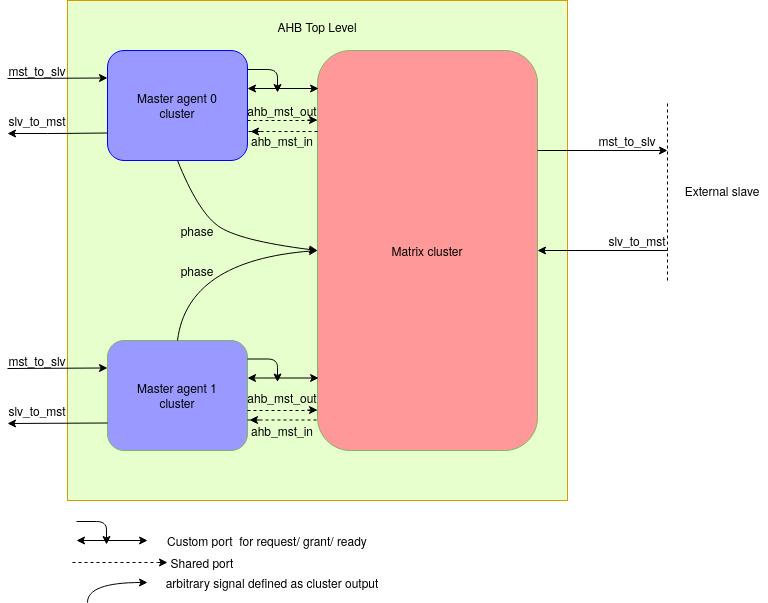
\includegraphics[width=8cm]{figs/Verif/Verif_block.png}
\caption{Verification clusters}\label{fig:verif-clust}
\end{wrapfigure} 

Fig.~\ref{fig:verif-clust} provides an overview of the verification clusters and their connections. I/O connections are listed with their compound names with port type indicated in the legend. The master agent is a relatively simple design so this section is mainly focused on the matrix cluster. The Gap Free Verification process introduced in Sec.~\ref{sub:gfv} is carried out on the matrix cluster. \par
It is not possible to determine every state of the matrix cluster by observing internal registers alone. There are no registers differentiating between a default master being idle or in the data phase of a transfer. Looking at signal values in the past require constraints on wait states. A better alternative is to define the state of the default master agent as an output to its cluster and an input to the matrix cluster. The states are determined based on this signal, address and data bus ownership as well as slave notify signals. \par
The first step is to define a Conceptual State Machine for the matrix cluster and write a set of skeleton properties to cover all core operations. Consider the FSM of the bus matrix from Sec.~\ref{sub:bus-matrix}, where the state \textit{Data} is divided into a set of conceptual states. Each communication over a blocking port signals an important state. The CSM of the matrix cluster, with the required minimum of conceptual states is listed below.    
 
\begin{enumerate}
 \item Idle: No transfer in progress, \textbf{HREADY} is set and bus is ready to accept a new request (1,2).
 \item Address: A transfer is initiated, \textbf{HREADY} is set and bus is ready to accept a new request.(3)
 \item Slave(x)\_write: Important state for each slave output. (4)
 \item Slave(x)\_read: Important state for each slave input (5)
 \item Data\_end: A transfer is completed, \textbf{HREADY} is set and bus is ready to accept a new request. (1,2,3) 
\end{enumerate}

Operation properties must cover all possible requests, read and write transaction to all slaves, success and error response from slaves as well a transaction to the default slave. Most properties have a duration of one time-point, with write transactions, error response from slave and default slave response covering two time-points. \par
The state of the bus is determined by address bus ownership, data bus ownership and which state the default master is in. Address and data bus ownerships are assigned to registers in the arbiter RTL module with the names \textit{master\_sel} and \textit{r\_master\_sel} respectively. The state \textit{Address} can be determined by checking that a single transfer is in progress and it is in the address phase.  
\begin{figure}[h!]
\begin{VHI}
macro Address_state : boolean :=
r_master_sel = 0 and agent0 /= data_phase and
(master_sel /= 0 or agent0 = address_phase)
end macro;
\end{VHI}
\caption{Address state condition, default master = 0}
\end{figure}

The state \textit{Data\_end} is determined in a similar fashion, except it is not concerned with any transfer possibly being in the address phase. The next state is decided by checking the address bus if a transfer is in progress and if there are any pending requests.
\begin{figure}[h!]
\begin{VHI}
macro Data_end : boolean :=
(r_master_sel /= 0 or agent0 = data_phase) and hready = true
end macro;
\end{VHI} 
\caption{Data\_end condition, default master = 0}
\end{figure}

The only visible registers required to hand over signal values between properties are the signals of the address bus, or more specifically the signals of the address bus which forms part of the payload, including \textbf{HTRANS}. The payload from a granted request is visible on the address bus and \textbf{HTRANS} indicates that a transfer is in progress. \textbf{HWDATA} is fetched directly from the interface of the appropriate agent before the entire payload is assigned the slave outputs. It may appear from line 4 in Fig.~\ref{fig:write-prop} that \textbf{HWDATA} is sampled in the address phase, but this is corrected in the signal macro using the "next" operator. 
\begin{figure}[h!]
\begin{VHI}
 for timepoints: t_end = t+2; 
 freeze:
   address_bus_haddr_at_t = address_bus_haddr@t,
   agentx_hwdata_at_t = agentx_hwdata@t; --next(agentx_hwdata)
 
 assume:
   at t: Address_state;
   at t: address_bus_haddr = slave0_range;
   at t: address_bus_hwrite = WRITE;
   at t: address_bus_owner = x; 
 
 prove:
   at t_end: slave0_write;
   at t_end: slave0_out_notify = true;
   at t_end: slave0_out_hwdata = agentx_hwdata_at_t;
   at t_end: slave0_out_haddr = address_bus_haddr_at_t;
   during[t+1,t_end]: hready = false; --always determined
\end{VHI}
\caption{Write property example}
\label{fig:write-prop}
\end{figure}

What remains is to determine the cluster outputs, which are all outputs to the master agents and slaves. All notify signals to the slaves and \textbf{HREADY} must be determined at all times. The remaining outputs should be determined conditionally. No signals on the master agent interface are sampled by the master agent unless \textbf{HREADY} is set. No signals on the slave interface are sampled by the slave unless its accompanying notify is set. \par 
This section has described the essentials for proving completeness on the matrix cluster for single transfers. Extended functionality such as burst transfers is discussed in Sec.~\ref{sec:burst}
 

\section{ESL}
After a complete set of abstract properties for the bus matrix is derived, the ESL model is developed. In the previous section it was established that master agents must be verified in separate clusters. This translates to the ESL by separating the master agents in their own SystemC-PPA module. Defining a suitable interface between the master agent and bus matrix requires careful consideration. \par
With blocking ports, correct simulation behavior and the highest level of abstraction is achieved, but that creates an issue with the bus matrix ESL module for multiple masters. Up to three blocking ports need to be serviced in the same time-point due to parallelism, which is not permitted in SystemC-PPA. A helper module is introduced which is not intended for property generation, but to serve as an emulated port interface. The requirements of this module are described in Sec.~\ref{sub:portem}.

\subsection{Bus matrix}
\label{sub:bus-matrix-design}
No more than three explicit states are required to model the bus matrix at the ESL. The implementation of the bus matrix ESL covered in Sec.~\ref{sub:bus-matrix} is elaborated with requirements and options. \par
The communication with the emulated port must occur as shown in Fig.~\ref{fig:em-port-code} exactly once in all three states. It is what signals the conceptual states 1,2 and 5 from Sec.~\ref{sec:bottom-up}. It is required to be a non-blocking write to unconditionally call a wait function, which hands over control to the emulated port so that the requests are updated before they are gotten. 
\begin{figure}[h!]
\begin{C++}
update_requests->try_write(true, sync, "state");  
requests_in->get(reqs); 
\end{C++}
\caption{Emulated port interaction}
\label{fig:em-port-code}
\end{figure}

The functionality of the arbitration scheme is carried out in cooperation between the bus matrix and the emulated port. It is essential that the arbitration scheme is modeled equally in the two modules. \par
Fixed-priority arbitration is the scheme chosen for this work, mainly due to its simplicity. It can be modeled with a simple if-else conditional statement that is easily transferable to the emulated port. The "else" clause starting at line 9 in Fig.~\ref{fig:arbitration-code} shows the control of the address bus falling back to the default master when no request is pending.

\begin{figure}[h!]
\begin{C++}
...
else if(reqs.m3_request){
 AS_regs = payload3; // assign address and control
 AS_regs.htrans = NONSEQ;
 addr_owner = 3;
else{
 AS_regs = payload0;
 AS_regs.htrans = IDLE;
 addr_owner = 0;
}
\end{C++}
\caption{Pseudo arbitration example}
\label{fig:arbitration-code}
\end{figure}

\textit{AS\_regs} only models signals on the address bus and does not include \textit{hwdata}. It is not practical to model \textit{hwdata} in such a way that a visible register mapping is required in the properties. Instead, the bus matrix differentiates read and write transfers when it transitions $Address\rightarrow Data$. Recall from Fig.~\ref{fig:data-fetch} how the payload data is fetched and subsequently written to the slave. Read transactions must write a zero value to the slave, to avoid the need to account for old values of \textit{hwdata} in each slave. \par
If the slave responds with an error, it is not sufficient to rely on the response payload to relay this information implicitly. The two-cycle error response adds an additional cycle, which must be proven in a separate property. Explicitly assigning the error as shown in line 3 of Fig.~\ref{fig:error-assign} ensures that separate properties are generated for the two different responses, which can be refined accordingly.  
\begin{figure}[h!]
\begin{C++}
slave(x)_to_bus->read(resp, "state");
if(resp.hresp = error){
 to_mAgent(x).hresp = error; //explicitly assign error
}else{
 to_mAgent(x).hresp = resp.hresp; //implicitly assign okay
}
to_mAgent(x).hrdata = resp.hrdata;
to_mAgent(x).hgrant = m(x)_grant;
bus_to_mAgent(x)->set(to_mAgent(x));
} //slave(x)_end        
  //else{default slave response}
update_requests->try_write(true, sync, "data_end");
\end{C++}
\caption{Error assignment}
\label{fig:error-assign}
\end{figure}

The slave response is broadcast to all master agents, which in this work is carried out through shared ports. The slave response can be forwarded through the emulated port, but with almost no return on investment. It is not done in this work to keep the emulated port minimal. The default slave response is given when no slave is selected, which is error status and zero data. \par
Line 8 of Fig.~\ref{fig:error-assign} shows how \textit{hgrant} is assigned an enum value. The emulated port is not sufficient for representing this signal for multiple master agents and is therefore assigned separately. The value assignment of this signal serve no functional purpose in the ESL model. A boolean value can be assigned if logic is added to set/reset all grants for every possible request.  \par
The transition from the state \textit{Data} is dependent on the address bus and pending requests. The master agent outputs are dependent on which slave is selected. To avoid the need to account for this in the generated properties, default values are assigned before the state transition. 
\begin{figure}[h!]  
\begin{C++}
if(AS_regs.htrans == NONSEQ){ 
 nextstate = Data;
 DS_regs = AS_regs;
 AS_regs = setAS_regs(requests, payloads); 
}else{
 AS_regs = setAS_regs(requests, payloads); 
 if(request) nextstate = Address;
 else nextstate = Idle;
}
to_mAgent(x) = default_values; //hrdata = 0, okay response
bus_to_mAgent(x)->set(to_mAgent(x));
\end{C++}
\caption{Next state selection}
\end{figure}

\newpage

\subsection{Master Agent}
\label{sub:magent-design}
The SystemC-PPA module of the master agent needs to cover all signals of the master agent interface. Some of these signals are represented in the event handling of the blocking ports. The control flow of a bus request and accompanying signals (\textit{hbusreq, hgrant, hready}) are modeled with a single blocking write as seen from line 3 of Fig.~\ref {fig:request-code}.
\begin{figure}[h!] 
\begin{C++}
if(state == request){
  //issue request, wait for grant
  mAgent_request->write(true, "request"); 
  nextstate = address;
}
\end{C++}
\caption{Issuing requests}
\label{fig:request-code}
\end{figure}

The address and control signals are written out on a shared port to be determined in the address phase of the transfer. The blocking write in line 5 of Fig.~\ref{fig:address-phase} models the agent waiting for \textit{hready} to be set. 

\begin{figure}[hbt] 
\begin{C++}
if(state == address){
  ahb_mst_out = payload; //address and control signals
  ahb_mst_out.htrans = NONSEQ
  mAgent_to_bus->set(ahb_mst_out); //Write address and control to bus
  bus_ready->write(true, "address_phase");
  nextstate = data;
}
\end{C++}
\caption{Address phase example}
\label{fig:address-phase}
\end{figure}

Rather than writing the entire payload to the bus in an instance, the individual payload elements are written in their respective phases both in the ESL and RTL to capture the protocol in operation properties. The state \textit{data} illustrates the need for a shared port to transmit the data payload. When the emulated port reads the blocking port in line 5 of Fig.~\ref{data-phase}, it signals the end of the data phase. The request is already processed by the slave, which means the data would not reach its target.
\newpage
\begin{figure}[h!]
\begin{C++}
if(state == data){
 ahb_mst_out.htrans = IDLE; 
 ahb_mst_out.hwdata = payload.hwdata; //Write data to bus
 mAgent_to_bus->set(ahb_mst_out); 
 bus_ready->write(true, "data_phase"); //hready = end of data phase
 bus_to_mAgent->get(ahb_mst_in); //get response payload
 nextstate = to_master;
}
\end{C++}
\caption{Data phase example}
\label{data-phase}
\end{figure}


 
\subsection{Emulated port}
\label{sub:portem}
The emulated port has strict requirements to ensure correct simulation behavior, both in terms of synchronization and in terms of arbitration. This module cannot be proven formally to be a sound abstraction of the RTL for the same reason that it is implemented. The chosen arbitration scheme must be manually verified to exactly match the arbitration scheme in the bus matrix. \par 
The port must wait for a synchronization signal from the bus matrix, perform request forwarding, service all applicable blocking ports and return to wait for a synchronization signal without interruption. This is accomplished by utilizing blocking inputs for both ports from each master agent, and performing a non-blocking read, only if there is a writer waiting. 
\begin{figure}[h!]
\begin{C++}
//begin while
update_requests->read(); 
//requests must be reset 
if(mAgent0_request->peek()){
mAgent0_request->try_read();
requests.m0_request = true;
}else if(mAgent1_request//....

requests_out->set(requests); 
if(bus_ready0->peek()) bus_ready0->try_read();
if(bus_ready1->peek()) bus_ready1->try_read();
//end while
\end{C++}
\caption{Emulated port, fixed-priority pseudo code}
\end{figure}

\section{Refining the Properties}
\label{sec:refine}
This section describes how the generated property sets are refined to hold on the design. Every I/O signal, visible register and important state is represented with a macro, which is of the form seen in Fig.~\ref{fig:macro}.
\begin{figure}[h!]
\begin{VHI}
macro signal_name : type := refinement end macro;
\end{VHI}
\caption{Signal macro}
\label{fig:macro}
\end{figure}

The next two sections describe the refinement of the signals, visible registers and states in the two clusters. The refinement of the signals representing the emulated port interface is explained for both clusters collectively in Sec.~\ref{sub:em-port-refine}.

\subsection{Bus Matrix}
All I/O signals of the bus matrix are refined to represent their similarly named top level RTL signal. There are, however, some signals that need some added logic. These are all signals which are represented at the ESL using enum values and signals which are not assigned values on a clock edge in the RTL. \par
One example which covers both scenarios is the signal \textbf{HSIZE} from the master agent. 
\begin{figure}[h!] 
\begin{VHI}
macro agentx_hsize : mask := 
if(next(agentx.hsize) = "000") then MT_B 
elsif(next(agentx.hsize) = "001") then MT_H 
------------------------------------------
property request_agentx is
 freeze: 
  agentx_hsize_at_t = agent0_hsize@t;
 
 assume: 
  at t: Idle_state;
  at t: agentx_request;

 prove: 
  at t_end: address_bus_hsize = agentx_hsize_at_t; --t_end = t+1
\end{VHI} 
\caption{Enum type refinement with next operator}
\label{fig:next-operator}
\end{figure}
Line 14 of Fig.~\ref{fig:next-operator} shows how the address bus signal is assigned a value from time $t$, whereas the address bus is actually updated with a signal from time $t\_end$. Line 1-3 shows how the "next" operator is used on the top-level RTL signal to assign the signal value from the next time-point and how the enum type is accounted for. \par
The output \textit{hgrant} is a similar issue, but in the opposite time direction. It can be determined at t\_end by assigning it the "prev" operator. In this work the choice is instead to assign it an enum value, to avoid unnecessary overhead at the ESL. The enum values \textit{m(x)\_grant} seen in Fig.~\ref{fig:agent-output} are defined as their own functions in the property set. The default master owns a grant when no other master does and therefore has a separate function. 
\begin{figure}[h!] 
\begin{VHI}
macro m(x)_grant : boolean :=
if(agentx_request and not(higher_prio_request) and hready) then true
elsif(addr_own = agentx and not(hready)) then true
else false 
end if;
end macro;
\end{VHI}
\caption{Function to determine \textbf{HGRANTx}}
\end{figure}

The visible registers are the address bus signals and ownership, which are mapped to the physical signals in the arbiter RTL module. The data bus ownership is required to determine some states, but it is removed from the property set through optimizations done by the tool DeSCAM. Macros for this register and the default master state are added in the refinement process. \par
The state variables from the ESL description are included in the property set although their type and values represent abstract states. A type is added to the RTL signal package, which is never used except to map these state variables to. \par
The constant functions which assign the visible registers associated with the address bus have dedicated functions generated which prove these assignments. 


\subsubsection{Completeness Description}
All inputs, as well as the default master state are listed with their signal macro names as determination assumptions. \par
All outputs are listed as determination requirements, most of them conditionally. The unconditional signals are the following: \\

\begin{tabular}{p{4.3cm} | p{10cm}}
\textit{update\_requests\_notify} & Determines \textbf{HREADY} to all master agents. An assertion which proves that they always have the same value is added as dependency. \\
\hline
\textit{bus\_to\_slave(x)\_notify} & Shares the same name as the RTL signal \\
\textit{slave\_to\_bus(x)\_notify} &  \\
\end{tabular}

The top two signals are used as conditions to determine the remaining outputs. The slave outputs are determined if \textit{bus\_to\_slave(x)\_notify} is set and \textbf{HRDATA}, \textbf{HRESP} and \textbf{HGRANTx} are determined if \textit{update\_requests\_notify} is set. \par

The visible registers for the address bus and address bus ownership are listed as local determination requirements. The data bus ownership is not listed here, because it is optimized away from the property set. It is not used to directly determine any outputs so it can be left out without failing any determination checks, although it would ideally be covered by the property set as an added precaution. \par

\subsection{Master Agent}
The property set and completeness description is identical for all master agents, therefore it is only refined for one master. 
All I/O signals except the emulated port interfaces are refined with their similarly named top-level RTL signal. In the master agent, \textit{hsize} is an output, so the signal is therefore determined as seen for \textit{hsize} in the bus matrix, an assertion is added to prove this correspondence. \par
The registers storing the requests are refined to mAgent0/(xx)\_reg. All states are refined to the corresponding state of the RTL design.\par
The completeness description lists all inputs and outputs with the signal macros generated from the SystemC-PPA. The emulated port interfaces are sufficient to determine all signals used within the macros. The state of the agent is added as a determination requirement so that it can be used as an input to the matrix cluster. \par
It is worth mentioning that in a single master system, the wait properties related to the states \textit{request} and \textit{address} have unreachable witnesses. The scenario where the master agent waits here never occurs. 

\subsection{Emulated port interface}
\label{sub:em-port-refine}
The blocking interface in the ESL model has a set of signal macros generated for each port to verify the four-phase handshake in the RTL model.
\begin{figure}[h!]
\begin{VHI}
blocking_out_notify : boolean := refinement end macro; --event notify
blocking_out_sync : boolean := refinement end macro;   --wait(event)
blocking_out_sig : type := refinement end macro;       --payload
\end{VHI}
\caption{Blocking port macros}
\end{figure}

The emulated port interfaces mostly use the sync and notify to convey information. Some of these do not exist in the RTL design, so they are given abstract values to satisfy the properties. Following is a pseudo refinement of the existing signals. 

\begin{figure}[h!]
\begin{VHI}
--master agent
macro agent0_request_notify : boolean := hbusreq0 end macro;
macro agent0_request_sync : boolean := hgrant0 and hready0 end macro;
macro agent0_ready_sync : boolean := hready0 end macro;

-- bus matrix
macro update_requests_notify : boolean :=
 hready0 and hready1 or --example with two masters
 hready0 and hgrant0 or
 hready1 and hgrant1
end macro;

macro requests_in_sig_m0 : boolean := hbusreq0 end macro;
macro requests_in_sig_m1 : boolean := hbusreq1 end macro;
\end{VHI}
\caption{Refinement of emulated port interfaces}
\label{fig:em-port-refine}
\end{figure}

Fig.~\ref{fig:em-port-refine} shows how the connections between the top-level signals are represented on each side of the port. The signal in line 2 corresponds with the signal in line 13. The signals from line 8-10 correspond to the signals of lines 3 and 4. As long as the logic described in the macro of line 7-11 is guaranteed within the emulated port it should not leave a gap in verification. However, this representation is not sufficient to use in the completeness description to determine \textbf{HGRANTx} as output. The macros generated from the shared ports are used in the completeness description for these signals in addition. 
  

\section{RTL}
The open source architecture used in this work is defined in one architectural module; \textit{ahb\_arbiter.vhd}. It uses arbitration functions from the file \textit{ahb\_func.vhd}, slave address configurations from \textit{ahb\_configure.vhdl}, packages from \textit{ahb\_package.vhd} and components from \textit{ahb\_component.vhdl}. \par
All payloads and state machine declarations used in the agents are added to the package file, as well as the unused type representing the ESL states of the bus matrix. It also contains some constants to offer readability for the signals which are hardwired. \par
Component declarations of all system modules are added to the component file, this includes agents, arbiter and bus matrix. The bus matrix is a top-level module for the arbiter, which instantiates the arbiter and provides default master selection and master priority. Master zero is highest priority, with priority decreasing with incrementing numbers. For simplicity, the highest priority master is set as the default in this work. \par
The configuration file contains the slave address ranges in decimal number, as well as the remapped address ranges of the slaves. Remap is not implemented in this work so they must be equal, remap is hardwired to zero for extra security. \par
The top-level module must include the following: \textit{library ieee}, \textit{logic\_1164} and \textit{numeric\_std} from ieee, \textit{ahb\_package} and \textit{ahb\_components}. \par
The arbiters reset is active low, so the top-level reset must be inverted before assigning it to the matrix port map. All slave agents require their address offset as a generic in the form of a 32-bit logic vector. All master and slave agents are connected to their inputs and outputs of the matrix with corresponding numbers. 

\subsection{Slave Agent}
The slave agent includes the same packages as the top-level, except for the components. It includes an additional package \textit{std\_logic\_unsigned} so that the slave address offset can be subtracted from the \textbf{HADDR} input. \par
\begin{wrapfigure}[12]{l}{6cm}
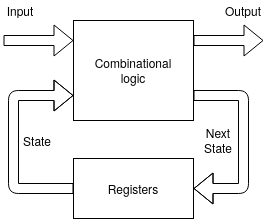
\includegraphics[width=5cm]{figs/hw/statemachine.png}
\caption{State machine}\label{fig:statem}
\end{wrapfigure} 

The slave agent is implemented as a state machine where combinational logic decides the next state based on internal registers and inputs. The state transitions are covered in Sec.~\ref{sub:sagent} and will not be reiterated here. What is covered is how the output assignments are handled so that properties can be generated from an ESL description which can be refined to hold on the design. These outputs are the request and response payload signals. \par
The request payload is stored in output registers after they are sampled in the address phase. When the signals are stored, the address offset is subtracted from \textbf{HADDR} and \textbf{HWDATA} is zeroed. If it is a write transaction, \textbf{HWDATA} is overwritten with the data bus value in the following cycle. \par
The response payload is stored in response registers and a flag is set simultaneously. The slave agent waits for \textbf{HREADY} to be set and zeroes the response payload registers.  



\subsection{Master Agent}
The master agent uses the same type of state machine as the slave agent. The functionality of the master agent is mirrored in the ESL description. Flags are set before the transfer phases are initiated, which signal when the address, control and data is written to the bus. 


\section{Building the Generator}
The generator consists of two parts; the hardware generator and the plugin which generates and refines the property sets. The hardware generator takes number of masters and slaves as input arguments. It begins by checking that the input arguments are within the range 1-15 and reads a text file containing slave address ranges. The slave address ranges are stored in a map. The generator instantiates two classes with this data which generate the system at the RTL and ESL. The generator produces a text file with the same stored data, converted for use within the plugin. It continues to call the plugin with the bus matrix and master agent SystemC-PPAs in turn. The plugin reads the text file and distinguishes between the two SystemC-PPAs to generate a refined property set and completeness description for each. 

\subsection{Hardware generator}
The generator uses the slave input argument to decide how many lines of the address map text file to read. It recognizes the words "start" and "end" to determine the start and end of the range. A separate map is produced for the ESL and RTL generation to avoid the need to convert the address format on the fly. The classes which generate the ESL and RTL are so similar in structure and function that they will not be described separately. \par
A set of files are generated for each abstraction layer, which are files that are not static with respect to number of masters and slaves. All files such as agents, dummies for test bench and arbiter remain in the output folder untouched and must not be deleted or modified. \par
All files are generated with an output file stream which is assigned a function output. Each file has its own dedicated function which writes the module description to a local string stream. Each function uses the stored number of masters, slaves and address map to produce its module according to the requested configuration. 

\subsection{Plugin: PrintAHB}
The plugin starts by reading the plugin data text file, which contains number of masters and slaves, as well as slave address ranges. The slave address ranges were used in an earlier implementation, but are not removed from the plugin data in case they are needed in the future. The plugin checks the file name if it is the bus matrix or master agent and calls the appropriate function to generate the property files. \par
DeSCAM creates an abstract model of the SystemC-PPA which is stored in a C++ object. This object contains maps and objects which together store all I/O signals, all variables, the FSM, property-suite etc. The plugin iterates over the components of the abstract model to simultaneously generate and refine the property macros as well as property set and completeness description.

\subsubsection{Bus matrix}
The I/O signals of the ESL design and RTL are given the same names, which simplify the automatic property refinement. The plugin iterates over a port map, converts the abstract signal name to its corresponding RTL signal name and writes it to a string stream. The process is shown in the following example.
\begin{figure}[h!] 
\begin{C++}
stringstream ss;
for(auto dp: ps->getDpSignals)
 //iterates over I/O signals in the abstract model
 ss << "macro" << dp->getName(); // insert name
 ss << //insert datatype

 ss << dp->getName().substr(0, dp->getName().find("_sig"));
 //Signals share name up to the "_sig" component added by the tool

 ss << "end macro"; 
 }
\end{C++}
\caption{Name extraction from abstract model}
\end{figure}


Some signals require more elaborate refinements, as is covered in Sec.~\ref{sec:refine}. These signals are checked for with if-else statements and refined accordingly when found. \par

The property refinement is carried out as follows:
\begin{itemize}
 \item I/O signals are refined as described above.
 \item The required assertions and macro functions are added for the appropriate number of masters. The macros for data bus ownership and default master state are subsequently added. 
 \item The visible registers do not share signal names with the RTL design, so every register is checked for by name and refined accordingly.
 \item The states are given recognizable names and numbering in the ESL model, which are transferred to the abstract model but with added numbering. The plugin iterates over the state map and refines the state macro according to name. If the state contains important numbering, this number is fetched with a function that excludes the numbering added by the tool.
 \item Each operation property is generated using functions which are slightly modified versions of functions from the plugin \textit{PrintITL} from \cite{descam}. Mainly, it modifies the time-points in the properties which require two cycles to complete by checking the assumptions and commitments.
 \item Two vacuous properties are removed from the property suite and completeness check by checking for a conflict between \textit{update\_requests\_sync} and \textit{not(requests)}.
\end{itemize}
\subsubsection{Master agent}
The master agent is refined to hold on master agent zero in a similar, but simpler, manner than the bus matrix. There are no vacuous properties which need to be removed. 



\section{Simulation}
\label{sec:sim}
\begin{figure}[hbt]
    \begin{center}
        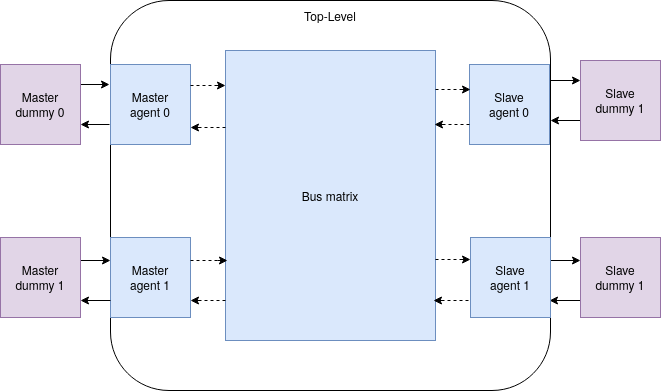
\includegraphics[width=0.7\textwidth]{figs/testbench.png}
    \end{center}
    \caption{Testbench block diagram, RTL example}
    \label{fig:testbench}
\end{figure}

Corresponding simulation models are generated for the RTL and ESL model. The simulation models offer a second layer of verification that the operations are carried out as intended and that the architecture behaves equally at both levels. \par
Master and slave dummies which carry out simple read and write operations are connected to the top-level design as seen in Fig.~\ref{fig:testbench}. The slave dummy has no knowledge of its address offset, or which master is operating it. Similarly, the master cannot distinguish if the slave it intended to access is the slave which is responding. VHDL does not offer the same high-level capabilities as C++, but the simulation models should operate on equal principles. This is accomplished by adding an identification number as input to the slave dummies in the RTL model and global functions to encode and decode identification numbers in both models. 

\begin{itemize}
 \item \textit{Write}: The master dummy calls a function from the included \textit{globals.h/.vhdl}, which takes target address as input argument and returns an ID number. The master adds this ID number to the top eight bits of its payload data. The slave dummy asserts that the top eight bits of the received data matches its own ID number. The ESL slave dummy must translate its object name to the corresponding ID number with a function available in the same included file. 
 \item \textit{Read}: The slave dummy adds its ID number to the top eight bits of its response data. The master dummy uses a function to assert that the response ID matches its target address ID.   
\end{itemize}  

The simulations are run for $10^6$ transfers, which are counted within the slave dummies, out of range transfers are therefore not counted and affects simulation time.  

\subsection{Starvation}
\label{sub:starvation}
One drawback of fixed-priority arbitration is that lower priority masters may never be granted access to the bus. When this occurs depend on the amount of masters, the rate of transfer for each master and the duration of each transfer. \par
Because starvation is inherently time-dependent some occurrences of starvation are not accurately captured in the untimed ESL simulation model. The rate of transfer depends not only on the rate of which a master writes to its agent, it also depends on whether the transfer is a write, read, successful or to the default slave. Furthermore, the delay within the masters and slaves play a part. \par
If all masters write as rapid as possible within the slave range, it is all but the three highest priority masters which starve in both models. If this shifts to outside the slave range, it is all but the four highest priority master which starve at the RTL, but the ESL remains the same. A similar discrepancy occurs if a delay is added between transfers in the masters and the transfer direction switches between read and write. \par
It is vital that an ESL simulation of a more elaborate system represent starvation adequately. The most important aspect of modeling starvation is that the ESL simulation does not show that a master can complete its task, when it actually starves forever in the RTL model. The two given examples indicate that the ESL simulation over approximates how many masters in the system are starving. If this is always true, the ESL model is sound when no masters are shown to starve during simulation. \par
Incrementing delays are temporarily inserted in the simulation models to provide some metrics for when starvation occurs. The masters are configured to wait for a certain time between each transfer, which is incremented after a certain number of transactions. When a master is granted access to the bus, it writes a message to the terminal which delay it required to receive a grant. The data for both models are shown graphically in Fig.~\ref{fig:starvation}. The ESL model is tested with different types of delays. The delays which are encountered in a real simulation model are wait statements called by port interfaces, which are either waiting for an event or for a certain time in picoseconds. Wait statements are also called when an important state is explicitly inserted. These wait statements cause a context switch and this thread is paused until the simulation has caught up with the time increment. \par
With random delays, the results are equal as with fixed delay if the amount of transfers between increments is high enough. For the random wait examples, the SystemC-PPA ports wait between one and $y$ picoseconds, whereas the masters wait between one and $x$ picoseconds. To reduce variability, $x$ is incremented after $5*10^5$ transactions.      

\begin{figure}[hbt]
\centering
\begin{subfigure}{.5\textwidth}
  \centering
  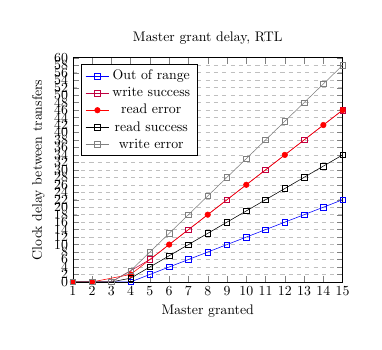
\begin{tikzpicture}[scale=0.5]
\begin{axis}[
    title={Master grant delay, RTL},
    xlabel={Master granted},
    ylabel={Clock delay between transfers},
    xmin=1, xmax=15,
    ymin=0, ymax=60,
    xtick={1,2,3,4,5,6,7,8,9,10,11,12,13,14,15},
    ytick={0,2,4,6,8,10,12,14,16,18,20,22,24,26,28,30,32,34,36,38,40,42,44,46,48,50,52,54,56,58,60},
    legend pos=north west,
    ymajorgrids=true,
    grid style=dashed,
]
\addplot[
    color=blue,
    mark=square,
    ]
    coordinates {
    (1,0)(2,0)(3,0)(4,0)(5,2)(6,4)(7,6)(8,8)(9,10)(10,12)(11,14)(12,16)(13,18)(14,20)(15,22)

    };
    \addlegendentry{Out of range}

\addplot[
    color=purple,
    mark=square,
    ]
    coordinates {
    (1,0)(3,0)(5,6)(7,14)(9,22)(11,30)(13,38)(15,46)

    };
    \addlegendentry{write success}

\addplot[
    color=red,
    mark=*,
    ]
    coordinates {
    (1,0)(2,0)(4,2)(6,10)(8,18)(10,26)(12,34)(14,42)(15,46)

    };
    \addlegendentry{read error}

\addplot[
    color=black,
    mark=square,
    ]
    coordinates {
    (1,0)(2,0)(3,0)(4,1)(5,4)(6,7)(7,10)(8,13)(9,16)(10,19)(11,22)(12,25)(13,28)(14,31)(15,34)
    };
    \addlegendentry{read success}

\addplot[
    color=gray,
    mark=square,
    ]
    coordinates {
    (1,0)(2,0)(3,0)(4,3)(5,8)(6,13)(7,18)(8,23)(9,28)(10,33)(11,38)(12,43)(13,48)(14,53)(15,58)

    };
    \addlegendentry{write error}

\end{axis}
\end{tikzpicture}
  \label{fig:sub1}
\end{subfigure}%
\begin{subfigure}{.5\textwidth}
  \centering
  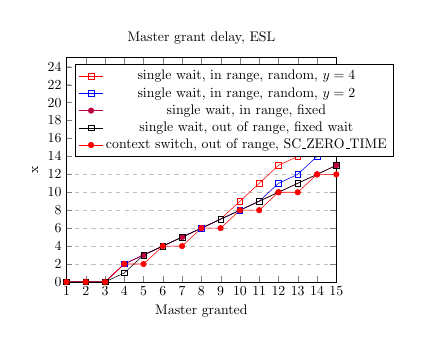
\begin{tikzpicture}[scale=0.5]
\begin{axis}[
    title={Master grant delay, ESL},
    xlabel={Master granted},
    ylabel={x},
    xmin=1, xmax=15,
    ymin=0, ymax=25,
    xtick={1,2,3,4,5,6,7,8,9,10,11,12,13,14,15},
    ytick={0,2,4,6,8,10,12,14,16,18,20,22,24},
    legend pos=north west,
    ymajorgrids=true,
    grid style=dashed,
]

\addplot[
   color=red,
    mark=square,
    ]
    coordinates {
    (1,0)(2,0)(3,0)(4,2)(5,3)(6,4)(7,5)(8,6)(9,7)(10,9)(11,11)(12,13)(13,14)(14,21)(15,22)

    };
    \addlegendentry{single wait, in range, random, $y=4$}

\addplot[
   color=blue,
    mark=square,
    ]
    coordinates {
    (1,0)(2,0)(3,0)(4,2)(5,3)(6,4)(7,5)(8,6)(9,7)(10,8)(11,9)(12,11)(13,12)(14,14)(15,16)

    };
    \addlegendentry{single wait, in range, random, $y=2$}



\addplot[
   color=purple,
    mark=*,
    ]
    coordinates {
    (1,0)(2,0)(3,0)(4,2)(5,3)(7,5)(8,6)(10,8)(12,10)(14,12)(15,13)

    };
    \addlegendentry{single wait, in range, fixed}


\addplot[ 
  color=black,
    mark=square,
    ]
    coordinates {
    (1,0)(2,0)(3,0)(4,1)(5,3)(6,4)(7,5)(9,7)(11,9)(13,11)(15,13)

    };
    \addlegendentry{single wait, out of range, fixed wait}

\addplot[ 
  color=red,
    mark=*,
    ]
    coordinates {
    (1,0)(2,0)(3,0)(4,2)(5,2)(6,4)(7,4)(8,6)(9,6)(10,8)(11,8)(12,10)(13,10)(14,12)(15,12)

    };
    \addlegendentry{context switch, out of range, SC\_ZERO\_TIME}


\end{axis}
\end{tikzpicture}
  \label{fig:sub2}
\end{subfigure}
\caption{Starvation comparison of RTL vs ESL}
\label{fig:starvation}
\end{figure}

Some measurements are not shown in the ESL portion of Fig.~\ref{fig:starvation} to keep the graph readable. The measurement for "context switch, in range  \textit{SC\_ZERO\_TIME}" and "context switch, in range, fixed"  are identical to the "single wait, in range, fixed" measurement. 
Fig.~\ref{fig:starvation} shows that it is not safe to assume that the ESL model over approximates how many masters starve. Foremost, if simulation time were equal to clock cycle time, master number four would receive a grant too early in the case of a write transaction. Additionally, there are no guarantees that a given amount of simulation time or context switches in the ESL model equates to a certain amount of clock cycles in the RTL. There is, however, a strong indication that the implementation of a monitor is feasible. The monitor can provide warnings or even halt the simulation if the model is not guaranteed to be sound. It can be implemented for fixed and random wait times, as long as \textit{SC\_ZERO\_TIME} is not intermixed with non-zero wait times.     


\section{Experimental Results}
 
Comparisons are made between the RTL model and its SystemC-PPA representation, to determine the efficacy of the abstraction. Tab.~\ref{tab:stats} compare the system components required of the different models with respect to configuration size. The variables listed in the PPA section are data path variables available in the abstract model and does not count intermediate variables used in the ESL model. One additional input and one visible register are added to the property set during the refinement process, which are not listed in the table. 

\begin{table}[hbt] 
  \begin{tabular}{ l r r r r r}
  \hline 
  \hline
      & \multicolumn{2}{c}{\textbf{\_\_\_}RTL\textbf{\_\_\_}} & \multicolumn{3}{c}{\textbf{\_\_\_\_\_\_}PPA\textbf{\_\_\_\_\_\_}} \\
   & inp./out. & FFs & inp./out & var. & states \\
    \hline
  AHB & - & 114 & - & 5 & 3 \\
  
  Per slave & 107/114 & 193 & 1/1 & - & 2 \\
 
  Per master & 107/114 & 286 & 2/4 & 12 & 5 \\
    \hline
    \hline  
  \end{tabular}
\caption{AHB system component comparison}
\label{tab:stats}
\end{table}

The difference in system components required to represent the same system level behavior is formidable. Comparing the input/output components between the two models for a system configuration of three masters and 15 slaves makes this evident. The RTL model utilizes a total of 1926 inputs and 2052 outputs whereas the ESL model utilizes 21 inputs and 27 outputs. The effect of this abstraction is seen when comparing the simulation time between the two models \par 
The simulation models introduced in Sec.~\ref{sec:sim} were run on a range of configurations of both models. The simulations are timed in seconds from start until a total of $10^6$ transactions are completed across the bus. The ESL configurations were run with cmake3, whereas the RTL configurations were run with Modelsim SE-64 10.7c. All simulations were run on the same computer within the span of hours, with no other programs running. The RTL simulations were run without adding any signals to the waveform display. The results are shown in Fig.~\ref{fig:simcompare} 
\newpage 

\begin{figure}[hbt]
\begin{center}
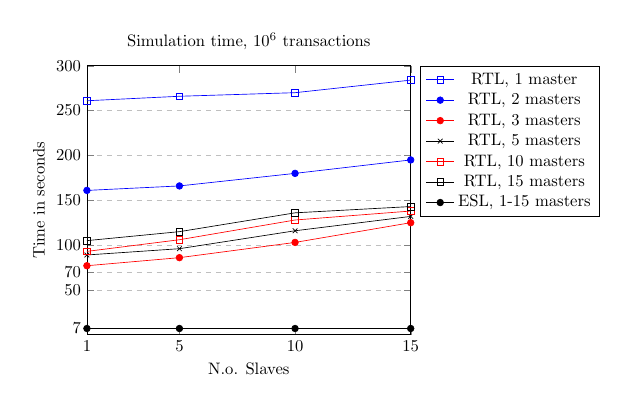
\begin{tikzpicture}[scale=0.6]
\begin{axis}[
    title={Simulation time, $10^6$ transactions},
    xlabel={N.o. Slaves},
    ylabel={Time in seconds},
    xmin=1, xmax=15,
    ymin=0, ymax=300,
    xtick={1,5,10,15},
    ytick={7,50,70,100,150,200,250,300},
    legend pos=outer north east,
    ymajorgrids=true,
    grid style=dashed,
]
\addplot[
    color=blue,
    mark=square,
    ]
    coordinates {
    (1,261)(5,266)(10,270)(15,284)

    };
    \addlegendentry{RTL, 1 master}

\addplot[
    color=blue,
    mark=*,
    ]
    coordinates {
    (1,161)(5,166)(10,180)(15,195)
    };
    \addlegendentry{RTL, 2 masters}

\addplot[
    color=red,
    mark=*,
    ]
    coordinates {
    (1,77)(5,86)(10,103)(15,125)
    };
    \addlegendentry{RTL, 3 masters}

\addplot[
    color=black,
    mark=x,
    ]
    coordinates {
   (1,89)(5,96)(10,116)(15,132)
    };
    \addlegendentry{RTL, 5 masters}

\addplot[
    color=red,
    mark=square,
    ]
    coordinates {
    (1,93)(5,106)(10,128)(15,138)
    };
    \addlegendentry{RTL, 10 masters}

\addplot[
    color=black,
    mark=square,
    ]
    coordinates {
    (1,105)(5,115)(10,136)(15,143)
    };
    \addlegendentry{RTL, 15 masters}
    
\addplot[
    color=black,
    mark=*,
    ]
    coordinates {
    (1,7)(5,7)(10,7)(15,7)
    };
    \addlegendentry{ESL, 1-15 masters}
\end{axis}
\end{tikzpicture}
\end{center}
\caption{Simulation comparison of RTL and ESL configurations}
\label{fig:simcompare}
\end{figure}

The RTL configurations with one or two masters show an increase in simulation time which is not proportional to the amount of system components from Tab.~\ref{tab:stats}. This offset in simulation time is due to the lack of parallelism within the master agents. When three or more masters work in parallel, the bus is utilized to its full potential. The ESL model is not affected by this lack of parallelism with respect to simulation time, nor is it affected by the size of the configuration. \par

The amount of properties generated depend exclusively on the number of slaves connected to the system. Assigning the address bus variables through constant functions reduce the amount of generated properties by up to 80\%. Two vacuous properties are removed during the refinement process and are not counted in the results. Fig.~\ref{fig:proof} shows the range of properties for all configurations, as well as total proof time for selected configuration sizes. The total proof time includes the completeness check. The master agent yields a property count of 11 regardless of configuration size.  
\newpage    

\begin{figure}[hbt]
\centering
\begin{subfigure}{.5\textwidth}
  \centering
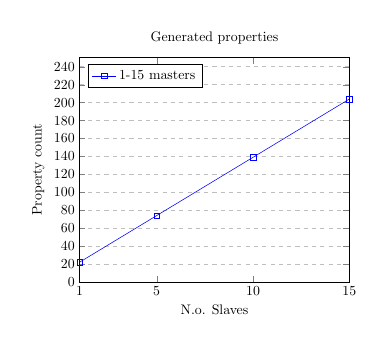
\begin{tikzpicture}[scale=0.5]
\begin{axis}[
    title={Generated properties},
    xlabel={N.o. Slaves},
    ylabel={Property count},
    xmin=1, xmax=15,
    ymin=0, ymax=250,
    xtick={1,5,10,15},
    ytick={0,20,40,60,80,100,120,140, 160, 180, 200, 220, 240},
    legend pos=north west,
    ymajorgrids=true,
    grid style=dashed,
]
\addplot[
    color=blue,
    mark=square,
    ]
    coordinates {
    (1,22)(5,74)(10,139)(15,204)

    };
    \addlegendentry{1-15 masters}


\end{axis}
\end{tikzpicture}
\label{fig:sub3}
\end{subfigure}%
\begin{subfigure}{.5\textwidth}
  \centering
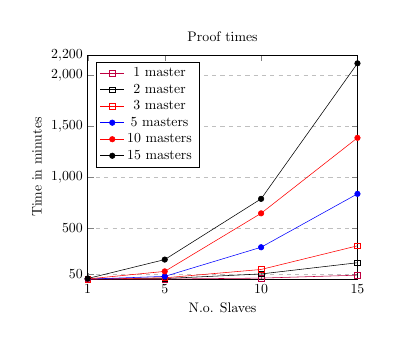
\begin{tikzpicture}[scale=0.5]
\begin{axis}[
    title={Proof times},
    xlabel={N.o. Slaves},
    ylabel={Time in minutes},
    xmin=1, xmax=15,
    ymin=0, ymax=2200,
    xtick={1,5,10,15},
    ytick={50,500, 1000, 1500, 2000, 2200},
    legend pos=north west,
    ymajorgrids=true,
    grid style=dashed,
]
\addplot[
    color=purple,
    mark=square,
    ]
    coordinates {
    (1,1)(5,2)(10,11)(15,40)

    };
    \addlegendentry{1 master}

\addplot[
    color=black,
    mark=square,
    ]
    coordinates {
    (1,1)(5,7)(10,52)(15,162)

    };
    \addlegendentry{2 master}

\addplot[
    color=red,
    mark=square,
    ]
    coordinates {
    (1,1)(5,14)(10,96)(15,328)

    };
    \addlegendentry{3 master}

\addplot[
    color=blue,
    mark=*,
    ]
    coordinates {
   (1,1)(5,28)(10,314)(15,838)
    };
    \addlegendentry{5 masters}

\addplot[
    color=red,
    mark=*,
    ]
    coordinates {
    (1,3)(5,77)(10,647)(15,1388)
    };
    \addlegendentry{10 masters}

\addplot[
    color=black,
    mark=*,
    ]
    coordinates {
    (1,7)(5,193)(10,789)(15,2119)
    };
    \addlegendentry{15 masters}
    
\end{axis}
\end{tikzpicture}
\label{fig:sub4}
\end{subfigure}
\caption{Property count and total proof time}
\label{fig:proof}
\end{figure}

Fig.~\ref{fig:proof} shows a strong dependency between amount of masters in the configuration and proof time. The property proof is measured and run with a single core. The property check is highly parallelizable, however, although running the property check with multiple cores reduced the total perceived time, it increased the total measured time by a factor of five in one configuration. This is possibly due to the resource management of the server in which the property checks were run. For that reason, all configurations are run with a single core. A number of the properties for configurations with one or two masters are vacuous, or have a witness that is unreachable. This is due to the FSM of the ESL model, which always includes transition possibilities for configurations of three masters and above. This, as a result, reduces the total proof time of the configuration in relation to amount
of properties.
\section{Concept: Burst Transfers}
\label{sec:burst}
This section covers a demonstration of how a four-beat incremental burst is implemented with SystemC-PPA and how the properties are refined to hold on the design.
The property set does not prove completeness; however, it is elaborated on how this can be achieved. It is also discussed how the remaining burst transfer types can be implemented and the limitations. \par
In this demonstration, a system with one master and one slave is used. The system is constrained to stay within the slave address range so that the address does not increment across the slave boundary or activates the default slave response. 

\subsection{Extensions to the RTL}
The master and slave agents are extended to support a four-beat incremental burst transfer. It is not implemented support for early burst termination. Early burst termination is not applicable in a single master system, but is disabled regardless by selecting "fair" fixed-priority arbitration.  
 
\subsubsection{Master Agent}
\begin{wrapfigure}[11]{l}{6cm}
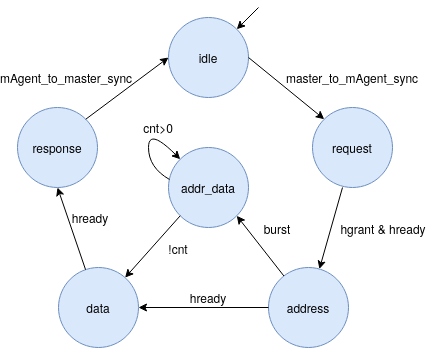
\includegraphics[width=5cm]{figs/hw/mAgent_burstfsm.png}
\caption{FSM with burst}\label{fig:magt-burstfsm}
\end{wrapfigure} 

An extra state \textit{addr\_data} is added to the state machine which carries out the concurrent clocking in/out of address and data. Data is clocked in or out using separate shift registers. Address is incremented by adding the address increment to the \textbf{HADDR} output. In this demonstration, a fixed data size of 32 bits is used. Two register banks are added as input and output between the agent and its master. Each register bank consists of four 32-bit registers which store the write or read burst data payloads. 

\subsubsection{Slave Agent}
\begin{figure}[hbt]
 \centering
 \begin{subfigure}[b]{0.4\linewidth}
 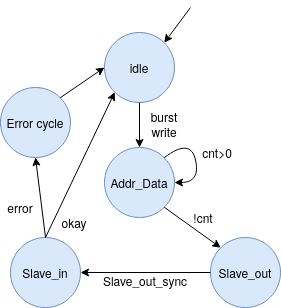
\includegraphics[width=0.7\linewidth]{figs/hw/sAgent_wburstfsm.png}
 \caption{burst write}
 \end{subfigure}
 \begin{subfigure}[b]{0.4\linewidth}
 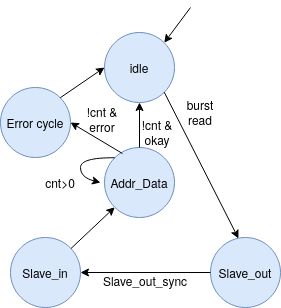
\includegraphics[width=0.7\linewidth]{figs/hw/sAgent_rburstfsm.png}
 \caption{burst read}
 \end{subfigure}
\caption{Slave agent FSM}
\label{fig:sagt-burstfsm}
\end{figure}

The slave agent state machine is more complicated. For this reason, single transfers are removed from Fig.~\ref{fig:sagt-burstfsm} and the burst write and read are shown in two separate figures for visibility. Register banks are added as inputs and outputs between the agent and its slave, including a register bank for the burst addresses. 
\begin{itemize}
 \item Burst write: Address and data are clocked in and written to the register banks. In the final beat of the burst, the slave agent samples the last data but still drives \textbf{HREADY} low to extend the transfer until it receives a response from the slave. The agent completes the transfer by driving \textbf{HREADY} high after response is received.
 \item Burst read: The slave agent samples the first address and immediately drives \textbf{HREADY} low to extend the transfer until it has received burst data from the slave. The slave must then calculate the remaining addresses internally using the control signals. When the agent receives the burst data payload, it drives \textbf{HREADY} high to clock the data out, and the remaining addresses in. This renders the address register bank redundant in the RTL module, but it is useful in property refinement.  
\end{itemize}

\subsection{Extensions to the ESL}
\begin{figure}[hbt]
    \begin{center}
        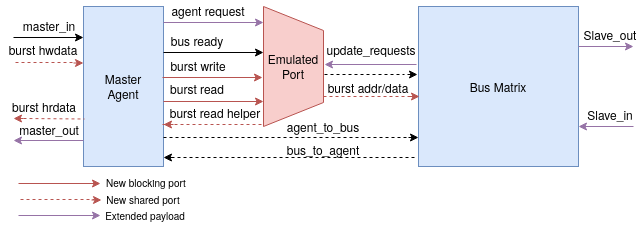
\includegraphics[width=0.8\textwidth]{figs/ESL/burst_esl.png}
    \end{center}
    \caption{ESL with burst added}
    \label{fig:esl-burst}
\end{figure}

The emulated port is not strictly necessary in a single master system; however, it remains in the demonstration to establish how bursts can be implemented for any configuration. In addition to the added ports shown in Fig.~\ref{fig:esl-burst}, some ports have extended their payload to account for burst transactions. One example of such a payload is shown in Fig.~\ref{fig:burst-resp-payload}. \par
 
\begin{figure}[h!] 
\begin{C++}
struct slv_out_burst_t{
    unsigned int hrdata0;
    unsigned int hrdata1;
    unsigned int hrdata2;
    unsigned int hrdata3;
    unsigned int hresp;
};
\end{C++}
\caption{Burst response payload}
\label{fig:burst-resp-payload}
\end{figure}
The payload in Fig.~\ref{fig:burst-resp-payload} represents all the response data of a four beat burst and is transferred in one instance at the ESL. In the property refinement, the individual \textit{hrdata} macros are time-shifted to match the data of the four separate beats of the burst in the RTL module.

When implementing burst transfers in SystemC-PPA modules, the generated properties must be considered. Each port interface is represented differently in the property set. Recall that blocking ports are accompanied with "sync" and "notify" signals, where no payload signals are determined in the properties unless the accompanying notify signal is set. This is practical in the macro refinement, since signals can be time-shifted without this causing issues for properties which are not concerned with the port in question. \par
Some payloads, like the payload in Fig.~\ref{fig:burst-resp-payload} are shared between all transfer types. The data variables which are not relevant for the transfer type are eliminated by assigning a zero value.  


\subsubsection{Master Agent}
\begin{wrapfigure}[13]{l}{6cm}
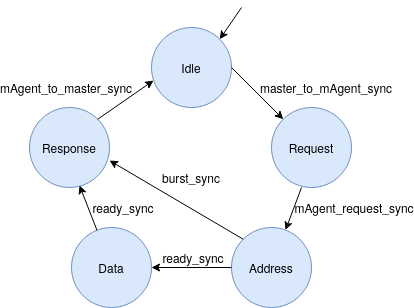
\includegraphics[width=5cm]{figs/ESL/mAgent_burstesl.png}
\caption{FSM with burst}\label{fig:magt-burstesl}
\end{wrapfigure} 

Fig.~\ref{fig:magt-burstesl} shows the FSM of the master agent with burst extension. The state \textit{addr\_data} is added to capture where the master agent is blocked pending the slaves burst read data. Transition conditions related to the \textit{bus\_ready} port are removed for readability, but its functionality remains as before. \par
The main challenge with burst transfers is assigning values to the $agent\rightarrow bus$ interface such that the address, control and data signals of the RTL model are represented throughout the transfer. The shared ports shown in Sec.~\ref{sub:magent-design} still represent the master agent interface for single transfers and must be accounted for during burst transactions as well, as seen in Fig.~\ref{fig:var-assign}. Note that variables displayed with a number range symbolize separate variables with corresponding numbers.
\newpage
\begin{figure}[h!]
\begin{C++}
payload.haddr = haddr+12;
payload.htrans = idle;
payload.hwdata = hwdata_shiftreg3;
agent_to_bus->set(payload); //assign values of final beat 

hwdata_shiftreg0 = hwdata_shiftreg3; //account for shifting
hwdata_shiftreg1-3 = 0;
\end{C++}
\caption{Internal signal, shared out assignment}
\label{fig:var-assign}
\end{figure} 


Single transfers operate as before with two exceptions. A helper payload is added to the \textit{agent\_request} port, which helps the emulated port distinguish between the transfer types. The response payload is extended to represent control signals for burst reads, which are eliminated for single transfers. \par
If the transaction is a burst write, the base address and data variables are assigned to the helper payload. The data variables must be transferred at an earlier stage to reach its target during simulation. The \textit{burst\_write} port only symbolically represent the data transfer for the generated properties. The $agent\rightarrow bus$ interface is represented for the entire transfer by adding every value to the payload. The sequence is represented by the assignment shown with pseudo code in Fig.~\ref{fig:burst-write-sequence}. Note that variables displayed with a number range symbolize separate variables with corresponding numbers.        

\begin{figure}[h!]
\begin{C++}
burst_write_payload.htrans = seq | seq | seq | idle; //concatenated
burst_write_payload.hwdata0-3 = hwdata_shiftreg0-3;
burst_write_payload.haddr1-3 = haddr + 4,8,12; 
burst_write_payload.hbusreq = e; //1110
burst_write->write(burst_write_payload, "data phase burst");
\end{C++}
\caption{payload assignment, burst write}
\label{fig:burst-write-sequence}
\end{figure}


Determining the signals of the $agent\rightarrow bus$ interface during burst read transactions is different. It is not so simple to extend the payload of the \textit{agent\_to\_bus} shared interface. Signal elimination would require very elaborate conditions to avoid disrupting unrelated properties. Instead, the response payload to the master is extended to include these signals symbolically instead. Error responses affect the duration of the transfer and in turn the value assignment as well. The sequence is represented by the assignment shown with pseudo code in Fig.~\ref{fig:burst-read-sequence}.   
\newpage
\begin{figure}[h!]
\begin{C++}
burst_read->write(true, "addr_data"); //Block the agent
burst_read_helper->get(slave_payload);
if(error) 
response.htrans = seq | seq | idle | idle; // extra cycle
else
response.htrans = seq | seq | idle; 

response.haddr2-3 = haddr + 4,8;   
hrdata0-3 = slave_payload.hrdata0-3;
burst_hrdata->set(hrdata); 
\end{C++}
\caption{payload assignment, burst read}
\label{fig:burst-read-sequence}
\end{figure}

\subsubsection{Bus Matrix}
The payloads of all the blocking ports in the bus matrix are extended to include burst payloads. The shared port representing the $bus\rightarrow agent$ interface is treated in the same manner as the $agent\rightarrow bus$ interface in the agent. In single transfers, all irrelevant signals are eliminated before the payloads are written to their respective ports. \par
No additional states are added to the FSM of this module, however, the burst read transaction requires separate conceptual states in the properties to handle the transfer between the slave and the master agent as shown in Fig.~\ref{fig:burst-read-matrix}.
\begin{figure}[h!]
\begin{C++}
bus_to_slave0->write(slvOutBurst, "slave0_write");
 if(AS_regs.hburst == 3 && AS_regs.hwrite == AHB_READ){
 slave_to_bus0->read(slvInBurst, "slave_read_back_br");
    \\sequence assignment
 update_requests->try_write(true, sync, slvInBurst, "Data_end_br")
 }
\end{C++}
\caption{Matrix, burst read}
\label{fig:burst-read-matrix}
\end{figure}

\subsubsection{Property macros}
Signal macros are generated for every component of each payload used in the burst transactions. Two of these payloads are described with examples, which cover the necessary aspects. 
\newpage
First, a simplified example of a property representing a burst write in the master agent is given in Fig.~\ref{fig:burst-property}. Note that variables displayed with a number range symbolize separate variables with corresponding numbers.

\begin{figure}[h!]
\begin{VHI}
property burst_write is
 for timepoints: t_end = t+4;
 
 freeze: 
   hwdata_shiftreg0-3_at_t = hwdata_shiftreg0-3@t,
   agent_to_bus_haddr_at_t = agent_to_bus_haddr@t;

 assume: 
   at t: address_state;
   at t: hburst = 3; -- four beat incremental
   at t: hwrite = WRITE;

 prove: 
   at t_end: burst_write_hwdata0-3 = hwdata_shiftreg0-3_at_t;
   at t_end: burst_write_haddr1-3 = agent_to_bus_haddr_at_t + 4,8,12;
   at t_end: burst_write_hbusreq = e;
   at t_end: burst_write_htrans = 252; --seq & seq & seq & idle 
   during[t+1, t_end]: agent_request_notify = false;
   during[t+1, t_end-1]: burst_write_notify = false;
   at t_end: burst_write_notify = true;
\end{VHI}
\caption{Simplified, burst write property}
\label{fig:burst-property}
\end{figure}


The burst write payload in the master agent is the simplest example, as no signals need elimination. The values of the signal macros for the individual signals are all evaluated from the perspective of the time point $t\_end$. The duration of the transaction is known in advance and assigned to $t\_end$. The signal macros of the time-shifted to represent the signal value in their respective time points. A selection of the signals from Fig.~\ref{fig:burst-property} are refined in the following example. The signal type declaration is removed for space considerations.  

\begin{figure}[h!]
\begin{VHI}
macro burst_write_hwdata0 := prev(agent_to_bus.hwdata,3) end macro;
macro burst_write_hwdata1 := prev(agent_to_bus.hwdata,2) end macro;
macro burst_write_hwdata2 := prev(agent_to_bus.hwdata) end macro;
macro burst_write_hwdata3 := agent_to_bus.hwdata end macro;
macro burst_write_htrans :=
prev(agent_to..htrans,3) & prev(..htrans,2) & prev(..htrans) & htrans
end macro;
\end{VHI}
\caption{Macro refinement, burst write}
\label{fig:write-refine}
\end{figure}

The refinement of signal macros where signals are eliminated are slightly more complex, particularly when error cycles must be accounted for. This occurs for burst read transactions in the master agent and is shown in Fig.~\ref{fig:error-and-elimination}. Observe in Line 4 and 6 how the signal macro is refined to represent a signal in the opposite direction, thus enabling it to be determined also for burst read transfers. 

\begin{figure}[h!]
\begin{VHI}
macro master_out_sig_haddr2 : unsigned := 
if(hburst = "011" and hwrite = READ) then
if(prev(bus_to_agent.hresp) = error_resp) then
prev(agent_to_bus.haddr,4) --extra cycle
else
prev(agent_to_bus.haddr,3)
end if;
else
resize(0,32) --eliminated
end if;
end macro;

macro master_out_sig_haddr3 : unsigned :=
if(hburst = "011" and hwrite = READ) then
agent_to_bus0.haddr --unaffected by error
else
resize(0,32) --eliminated
end macro;
\end{VHI}
\caption{Macro refinement, burst read}
\label{fig:error-and-elimination}
\end{figure}

\subsubsection{Further implementation and completeness}
The remaining burst transfer types can be implemented using the same concept as described here. Separate conditions and signal assignment must be added to the ESL for each burst type. The burst payloads can be shared between the burst types, they are merely extended to account for the signals required to represent a 16-beat burst transaction. The signals which are irrelevant for transactions of fewer beats are eliminated as shown in this demonstration. To account for wrapping bursts and different data sizes, the address is incremented through a function. The duration of each transfer type must be known in advance, which places one limitation on the system. Incremental burst transfers of undefined length can therefore not be implemented. \par
To prove completeness with burst transfers implemented, the remaining signals of the $agent\leftrightarrow bus$ interface must be determined throughout the burst transactions. This is feasible, but two aspects must be considered: 
\begin{enumerate}
 \item Signals represented through notify events at the ESL: This includes \textbf{HBUSREQx} in the master agent, and \textbf{HREADY} in the bus matrix. Observe from line 18 in Fig.~\ref{fig:burst-property} how the request notify is required to stay false throughout the transfer. In the RTL model \textbf{HBUSREQx} remains asserted throughout the state \textit{addr\_data}. It must therefore be included in the burst payload and the request notify must be set to false throughout the burst transactions. The same applies to \textbf{HREADY} in the bus matrix, it must be added to the payload to be determined in every cycle.
 \item Payload signals during wait cycles: In Fig.~\ref{fig:error-and-elimination} it is shown two subsequent addresses. They are time-shifted such that there is a span of up to three time points where none of them are determined. This is due to the wait cycles inserted by the slave agent. These time points can be accounted for by adding duplicates of signals in the ESL model. This is a cumbersome process, so it is suggested to rather allow certain signals to be undetermined in the properties. The \textit{allow\_undetermined} operator can be used on signals which are known not to change during wait cycles. 
\end{enumerate}

The default slave response must be accounted for. It is not clear how this is accomplished in the master agent. It is not known to the master agent if the transfer in question will provoke a default slave response or not, so the duration of the transaction is not known beforehand. It is also not known if an error response comes from the default slave response or not. One suggestion is to check for errors before burst write transactions, and after burst read transactions. The slaves are configured such that error response is accompanied by non-zero data. The master agent can determine where the error comes from and terminate the burst early if it originates from the default slave. \par
How to determine the state of the default master in the bus matrix must also be considered. The properties are no longer exclusively of length t+1 in the master agent, so it cannot be determined as an output and input to the clusters without determining it at all time points. One solution is to use an encoding on a signal like \textbf{HPROT} when \textbf{HTRANS} is encoded with IDLE together with the encoding on \textbf{HTRANS} to determine the state of the default master.   


